\documentclass[a4paper]{report}

\usepackage{graphicx}
\usepackage{amsmath}

\begin{document}

\begin{titlepage}

\newcommand{\HRule}{\rule{\linewidth}{0.5mm}} % Defines a new command for the horizontal lines, change thickness here

\center % Center everything on the page

\HRule \\[0.4cm]
{ \huge \bfseries Human Gait Analysis}\\[0.4cm] % Title of your document
\HRule \\[1.5cm]

%----------------------------------------------------------------------------------------
%	HEADING SECTIONS
%----------------------------------------------------------------------------------------
\textsc{\large Report submitted in fulfillment of the requirements
for the Exploratory Project of\\ % Minor heading such as course title
\bfseries{Second Year, IDD}.}\\[0.5cm]
%----------------------------------------------------------------------------------------
%	TITLE SECTION
%----------------------------------------------------------------------------------------


 
%----------------------------------------------------------------------------------------
%	AUTHOR SECTION
%----------------------------------------------------------------------------------------

\begin{minipage}{0.4\textwidth}
\begin{flushleft} \large
\emph{Author:}\\
\bfseries Utsav Krishnan \\% Your name
\end{flushleft}
\end{minipage}
~
\begin{minipage}{0.4\textwidth}
\begin{flushright} \large
\emph{Supervisor:} \\
\bfseries Dr. Hari Prabhat \textsc{Gupta} % Supervisor's Name
\end{flushright}
\end{minipage}\\[1cm]

% If you don't want a supervisor, uncomment the two lines below and remove the section above
%\Large \emph{Author:}\\
%John \textsc{Smith}\\[3cm] % Your name

%----------------------------------------------------------------------------------------
%	DATE SECTION
%----------------------------------------------------------------------------------------

{\large April \ \ \ , 2017}\\[1cm] % Date, change the \today to a set date if you want to be precise



\includegraphics{pictures/collegeLogo.png}\\[1.0cm]

\textsc{\Large \bfseries Department of Computer Science and Engineering}\\[0.5cm] % Major heading such as course name
\textsc{\Large \bfseries Indian Institute of Technology (BHU) Varanasi}\\[0.5cm] % Major heading such as course name
%----------------------------------------------------------------------------------------


%	LOGO SECTION
%----------------------------------------------------------------------------------------

% 
\includegraphics{collegeLogo.png}\\[0cm] % Include a department/university logo - this will require the graphicx package


%----------------------------------------------------------------------------------------

\vfill % Fill the rest of the page with whitespace

\end{titlepage}

\newpage\null\thispagestyle{empty}\newpage

% new page 

{\center \bfseries
{\Huge Dedicated to} \\[1cm]
\emph{{\huge My parents, teachers,....}
}}
% new page
\newpage
{\center \bfseries
{\Huge \underline{Declaration}} \\[1cm]
} 
I certify that
\begin{enumerate}
	\item The work contained in this report is original and has been done by myself and the general supervision of my supervisor.\newline
	\item The work has not been submitted for any project.\newline
	\item Whenever I have used materials (data, theoretical analysis, results) from other
sources, I have given due credit to them by citing them in the text of the thesis
and giving their details in the references.\newline
	\item Whenever I have quoted written materials from other sources, I have put them \newline
under quotation marks and given due credit to the sources by citing them and
giving required details in the references.\newline
\end{enumerate}

\begin{minipage}{0.3\textwidth}
\begin{flushleft} \large
Place:IIT (BHU) Varanasi \\
 Date: \\% Your name
\end{flushleft}
\end{minipage}
~
\begin{minipage}{0.67\textwidth}
\begin{flushright} \large{
\bfseries{Utsav Krishnan}} \\
 IDD Student \\
Department of Computer Scrience and Engineering.\\ % Supervisor's Name
Indian Institute of Technology (BHU)\\ varanasi 
INDIA 221005.
\end{flushright}
\end{minipage}\\[1cm]

% new certificate page
\newpage
{\center \bfseries
{\Huge \underline{Certificate}} \\[1cm]
} 
{\center{\emph{This is to certify that the work contained in this report entitled \lq\lq Human Gait Analysis\rq\rq \ being submitted by {\bfseries Utsav Krishnan} (Roll No. {\bfseries 15074014}),
carried out in the Department of Computer Science and Engineering, Indian Institute
of Technology (BHU) Varanasi, is a bona fide work of our supervision.}}}\\[2cm]

\begin{minipage}{0.3\textwidth}
\begin{flushleft} \large
Place:IIT (BHU) Varanasi \\
 Date: \\% Your name
\end{flushleft}
\end{minipage}
~
\begin{minipage}{0.67\textwidth}
\begin{flushright} \large{
\bfseries{Dr. Hari Prabhat Gupta}} \\
Department of Computer Scrience and Engineering.\\ % Supervisor's Name
Indian Institute of Technology (BHU)\\ varanasi 
INDIA 221005.
\end{flushright}
\end{minipage}\\[1cm]

% new page Acknowledgements
\newpage
{\center{\Huge \bfseries {Acknowledgements}}}\\[2cm]
{\center I would like to express my sincere gratitude to my superviser Dr. Hari Prabhat Gupta.}\\[2cm]

\begin{minipage}{0.3\textwidth}
\begin{flushleft} \large
Place:IIT (BHU) Varanasi \\
 Date: \\% Your name
\end{flushleft}
\end{minipage}
~
\begin{minipage}{0.67\textwidth}
\begin{flushright} \large{
\bfseries{Utsav Krishnan}} \\
\end{flushright}
\end{minipage}\\[1cm]



% new page abstract
\begin{abstract}
In this project, we compare the biometric gait of the human body using accelerometer sensor present in the smartphone.\newline\newline
The accelerometer data are acquired while the phone is in the trousers pocket in fixed orientation.\newline\newline
Data is then analyzed in time domain where average gait cycle is extracted for both legs, and their similarity is evaluated using Dynamic Time Wrapping.
\end{abstract}

\tableofcontents

\listoffigures

% \listoftables

\chapter{Introduction}

\section{Overview}


Biometrics refers to metrics related to human characteristics. Biometric authentication authentication is used in computer science as a part of identification and access control[1]. \newline


There being mainly two sub discipline namely behavioral and physiological. Behavioral characteristics deals with gait, voice, rhythm and the latter deals with body size and shape like fingerprint, iris, DNA, etc.\newline

In this project work we focus on gait analysis. Human gait can be analyzed different way, the common being image processing and accelerometer based, this latter being used for this project..\\


\section{Motivation of the Research Work}


Biometric analysis can be of great use in medical field. There has been news of doctors using Fitbit to monitor patients heart beat in hospitals. It could be of great value to people who needs to keep track of their heart beat. \newline

Although there are many gadget similar to that, but they are costly and common people doesn’t considers investing in it. But almost every people have smartphone and even the basic ones these days have built in accelerometer. Here we use android app which logs accelerometer readings and process it to understand gait cycle and compare it with other leg.\newline

Variation arise in gait pattern of both legs when a person is ill or tired/not feeling well. This app can inform the subject if he/she needs to consult a doctor and more importantly being cost effective.
\newpage
\section{Organisation of the Report}
\begin{itemize}
\item Data acquisition and storage
\item Noise removal and smoothing 
\item Feature template extraction and arriving at conclusion
\end{itemize}

\chapter{Data Acquision and Storage}


\section{Data acquisition}
Data is acquired by accelerometer present in the smartphone. Data logging is triggered by the subject by pressing the start button and the smartphone is kept in the trouser’s pocket, in a fixed orientation. Such that the +Y axis, +Z axis and X axis of the smart phone points in top,forward,sideways direction respectively.\newline

Then the subject walks considerable distance with the phone kept in the pocket with each leg.
\section{Storage}

The data is saved in txt format, which can be easily read on the computer. Two options are provided for storing accelerometer data, either in internal storage or in the external storage.\newline

\begin{figure}
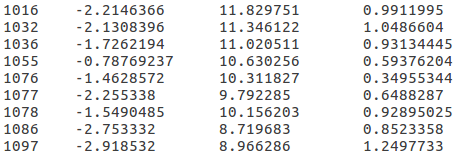
\includegraphics[width=100mm,scale=0.5]{pictures/recordedCrop.png}
\caption{The first, second, third and  fourth columns of the data log files are time, X-axis, Y-axis and  Z-axis respectively.}
\end{figure}

Each time data is recorded the data log file is overwritten.
We use sensor delay fastest for logging data. All three axis reading are stored in the log file.\newline

The app can also be used for standalone data logger.\newline

Only Z-axis is used here for further analysis. In this orientation we could have used both Z and Y axis effectively, but using X-axis is avoided because the time series graph obtained doesn’t provide meaningful gait cycle feature template.\\

\begin{figure}
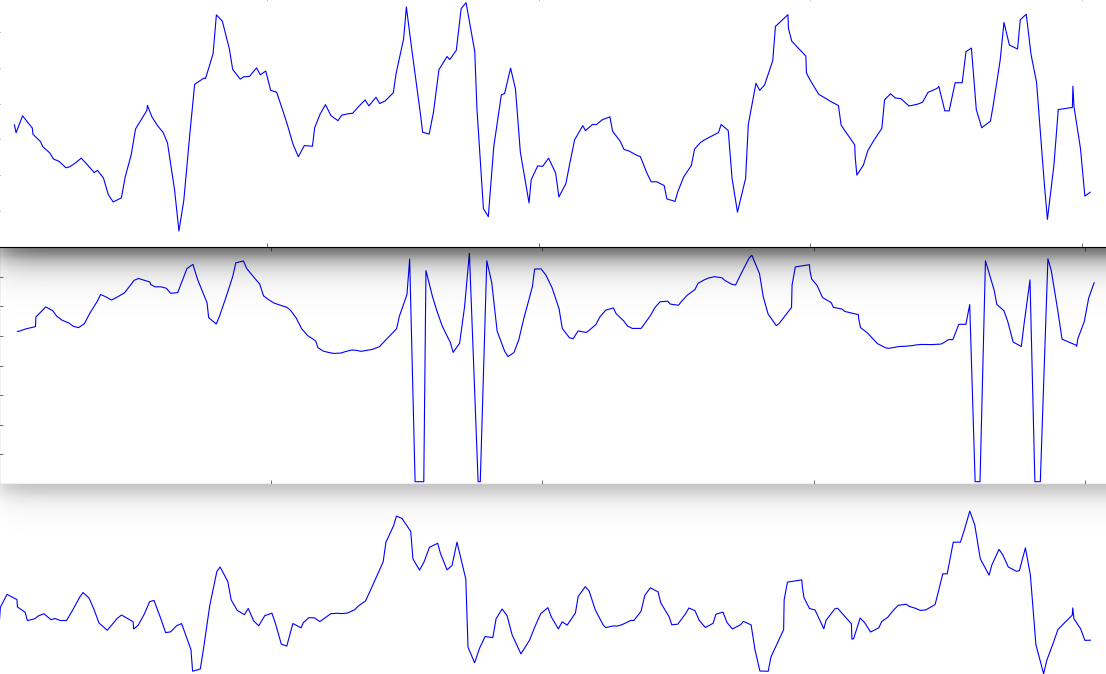
\includegraphics[scale=0.3]{pictures/XYZcrop.png}\\[1.0cm]
\caption{Raw X, Y, Z axis readings, from top to bottom. }
\end{figure}


\newpage
\chapter{Noise reduction and smoothing}
\section{Noise removal}

Following low-pass filter is used for removing high frequency noise from the data.\cite{lowpass}

The extent of filtering is set by the value of alpha as shown in the equation, the value of alpha represents the weight given to the previous data point called the inertia from the previous output.

\begin{verbatim}
   for i from 1 to n
       y[i] := y[i-1] + alpha * (x[i] - y[i-1])
\end{verbatim}

\begin{figure}
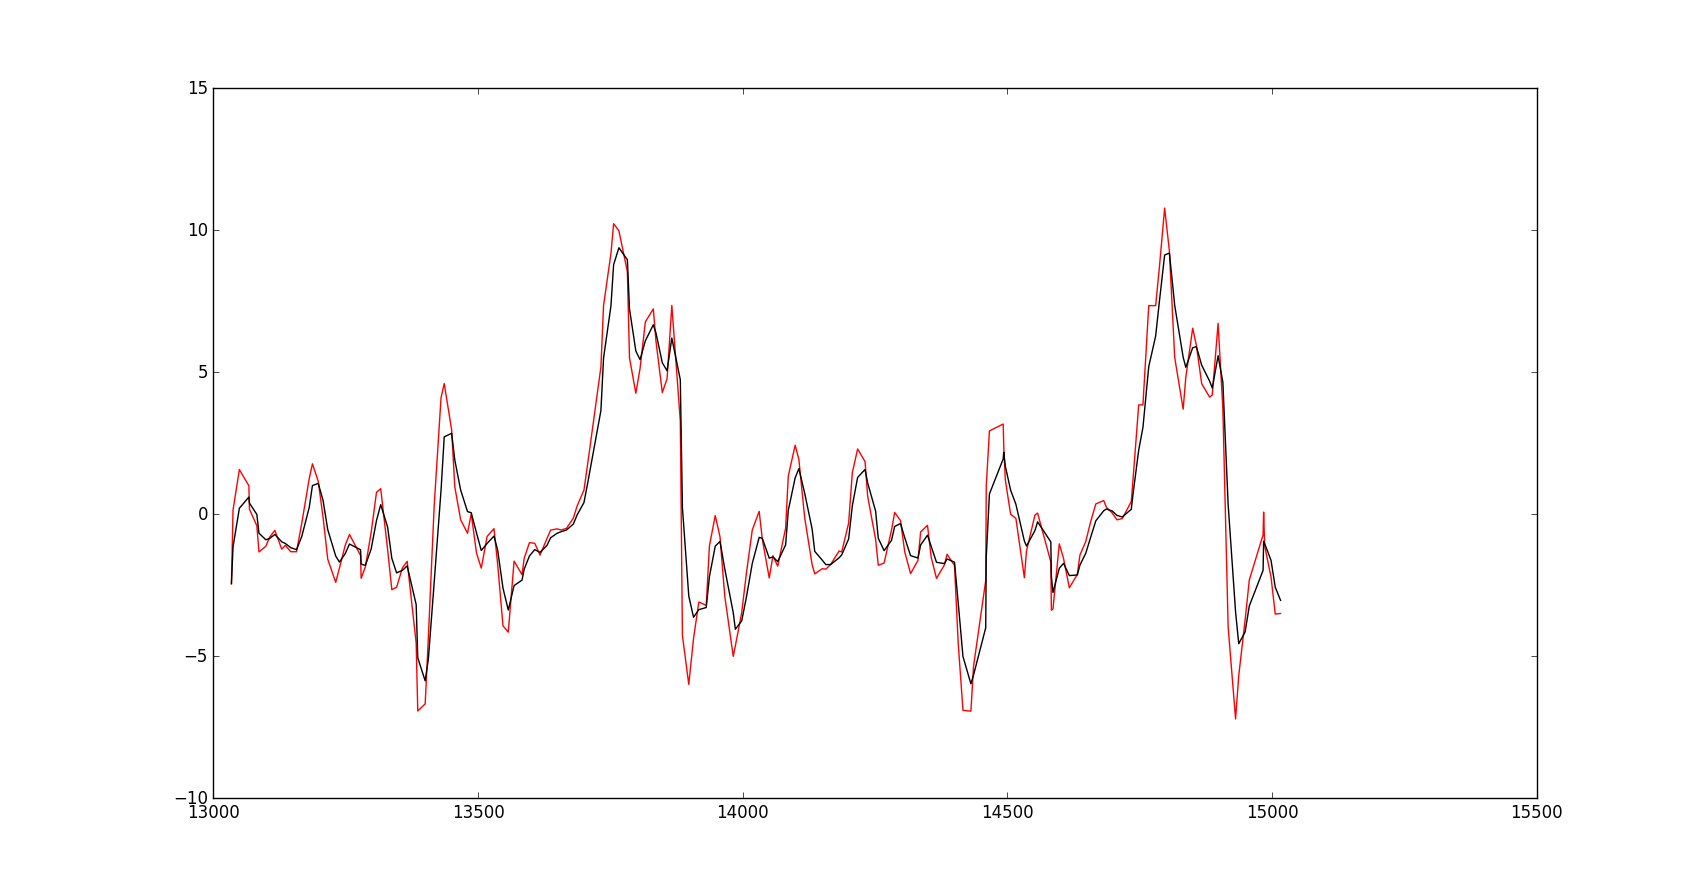
\includegraphics[scale=0.3]{pictures/LOWPASSfiltereddata.png}
\caption{Raw z-axis(red) readings vs low-pass filtered(black) data.}
\end{figure}


\section{Smoothing}
There being various method of smoothing, moving average was selected for our analysis, as it smooths the graph while maintaining the characteristic of the graph.\cite{ma} \newline

After many iterations the window size of 5 was chosen, if a large value of window size had been used then the variations could have not been so obvious. After experimenting it was also found out that running moving average 3-5 times with small window size proved to be better than running 1-2 window average with large window size as the gait cycle period points are short. \newline


The average of window size of data points are taken as average and the value is set to the median element. The weight given to every points in the window size over summation is the same.\newline
$$X_\frac{m+n}{2} = \frac{X_m + X_{m+1}+ \cdots + X_n}{n-m+1}
      = \frac{1}{n-m+1}\sum_{i=m}^{n} X_i$$

% algorithms for moving average can be included here
% \begin{verbatim}
%    for i from w/2 to n-w/2
%        y[i] := y[i-1] + alpha * (x[i] - y[i-1])
% \end{verbatim}
\begin{figure}
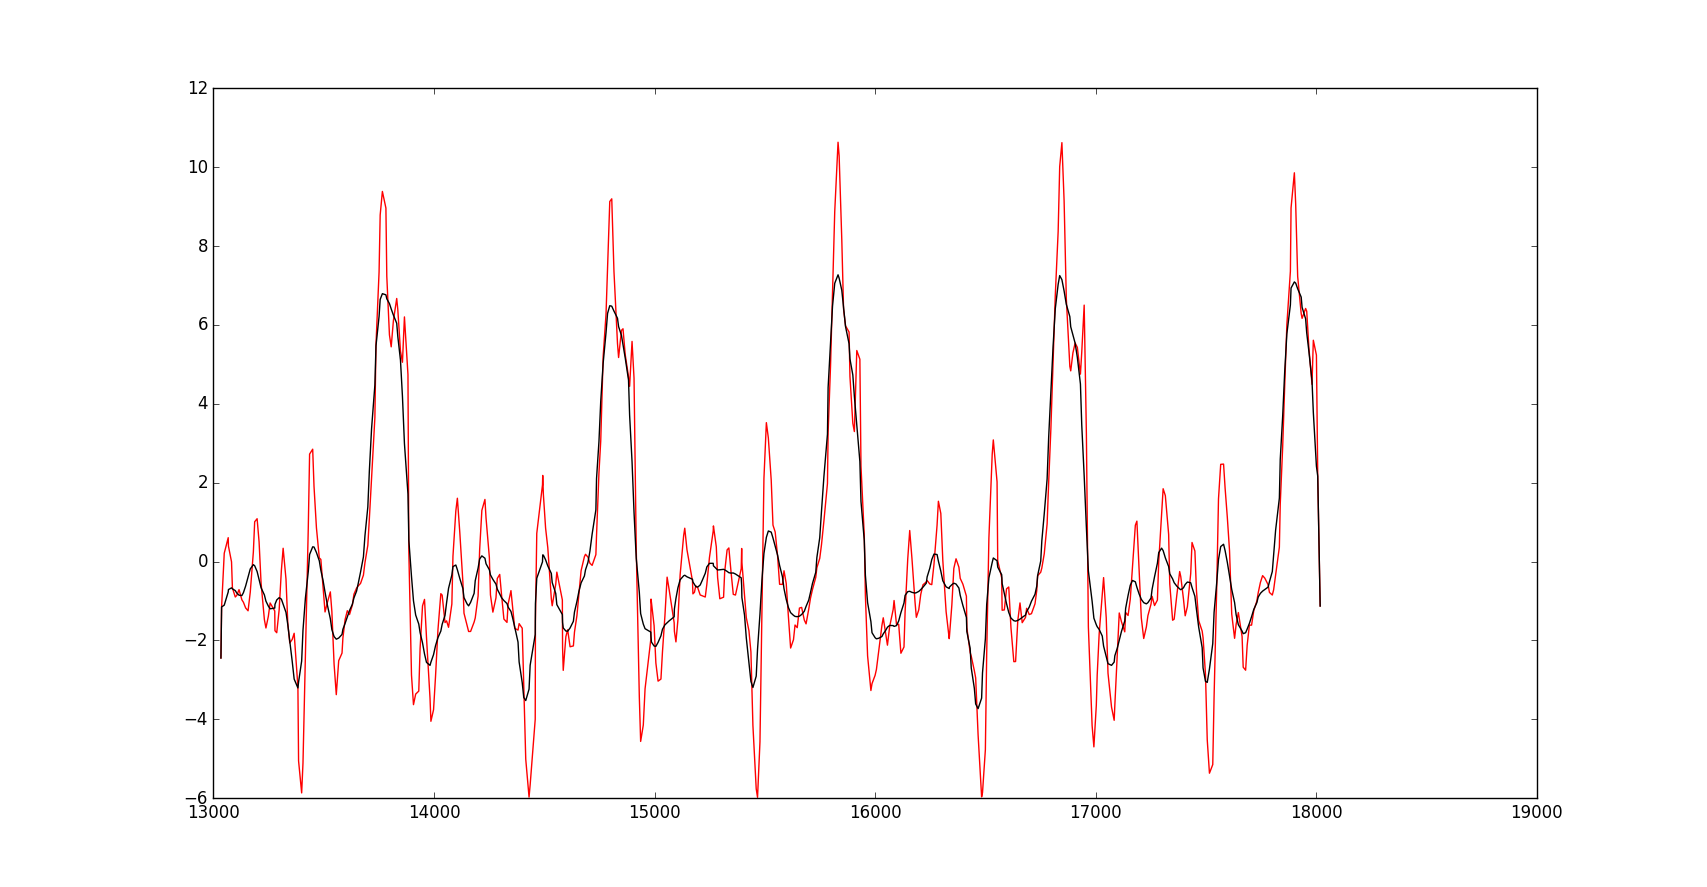
\includegraphics[scale=0.3]{pictures/maax3.png}
\caption{Moving Average applied on low-pass filtered data.}
\end{figure}

\section{Normalization}

Data is then normalized to reduce the distance between the maximum and minimum of 
gait cycle points while preserving the characteristics of the graph.\newline

$$ y = (x - min) / (max - min)\cite{normal} $$
\begin{figure}
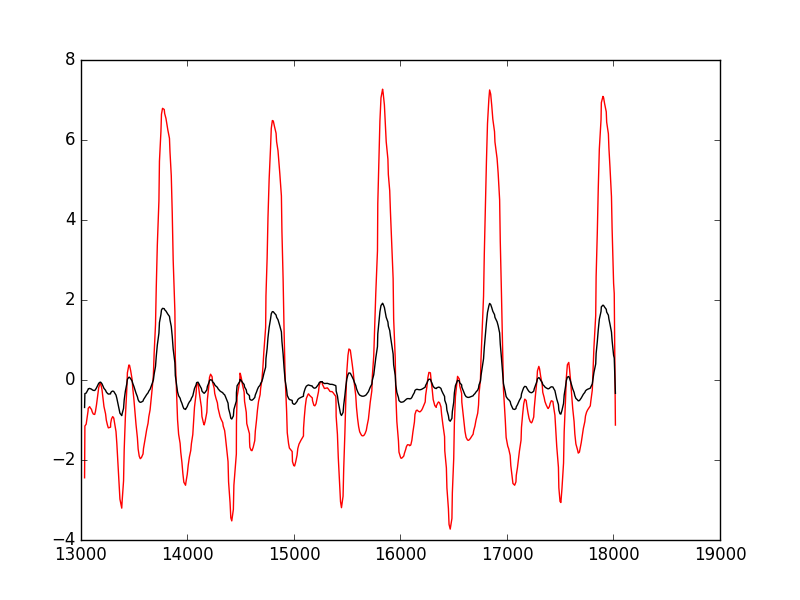
\includegraphics[scale=0.6]{pictures/normalized.png}
\caption{Normalization done on moving averaged data.}
\end{figure}

\newpage
\chapter{Feature Extraction}
\section{Maximal Points}
First all the points with local maxima are extracted, the points which are greater than its previous and next value. Then the points with value less than a threshold value is discarded. The threshold value is obtained from the equation[…….], where u is mean, sd is standard deviation and k is the whole number value set by the user. The value of k is found out by trial and error method, and depends from user to user.

\section{Gait Cycle Points} 
The remaining points forms the gait cycle[2]. cycle is sometimes called the walking cycle. It exists  between any two consecutive heel strike of the same leg[3].

\begin{figure}
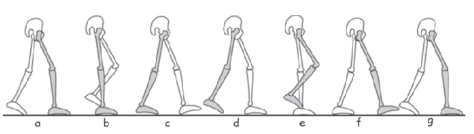
\includegraphics[scale=0.73]{pictures/gaitcycle.png}
\caption{Human Gait Cycle.}
\end{figure}

\subsection{Average Gait Cycle} 
Average Gait Cycle(AGC)[4] is defined as shown in the equation.
% \begin{equation*}
% AGC =
% \begin{cases}
% gaitcycle & | d_i = argmin(\frac{1}{N-1}\sum_{j\neq t}^{N} dtw_i,_j)\cite{dtw1}
% \end{cases}
% \end{equation*}


The term average could be misleading here as we are not taking average of all gait cycles,instead we compare each gait cycle with every other gait cycle and the one which has maximum resemblance to other gait cycles is considered as the average gait cycle.

It has an advantage, every extracted gait cycle may not be a gait cycle in reality instead it can be noise. Hence those noisy gait cycle will least resemble to other gait cycle and can not be a gait cycle. 

Had we been taken the average of all gait cycle the noisy gait cycle would have been considered distorting average gait cycle.

\begin{figure}
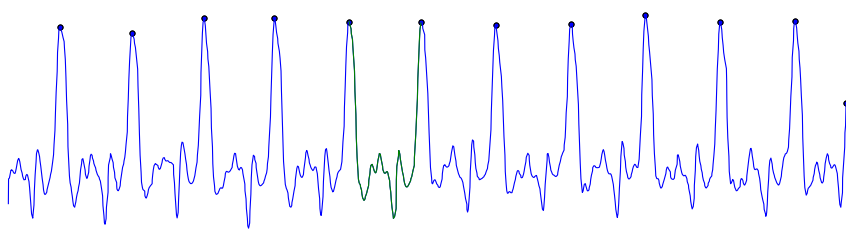
\includegraphics[scale=0.4]{pictures/agc_left_crop.png}
\caption{AGC of left leg(in black).}
\end{figure}

\begin{figure}
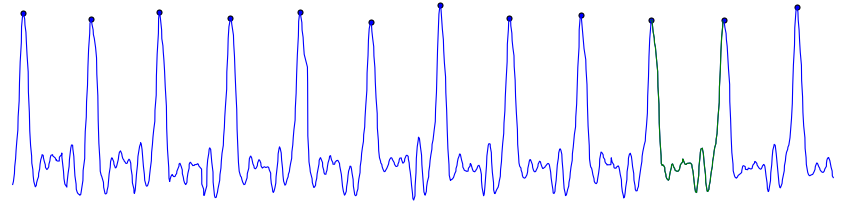
\includegraphics[scale=0.4]{pictures/agc_right_crop.png}
\caption{AGC of right leg(in black).}
\end{figure}


\section{Dynamic Time Wrapping}
The time domain technique that we used to compare any two gait cycle is Dynamic Time Wrapping(DTW)[5]. DTW is a pattern matching technique. We don’t have to normalize the length/duration of each gait cycle taking advantage of the property of DTW.


\begin{verbatim}
int DTWDistance(s: array [1..n], t: array [1..m]) {
   DTW := array [0..n, 0..m]

   for i := 1 to n
       DTW[i, 0] := infinity
   for i := 1 to m
       DTW[0, i] := infinity
   DTW[0, 0] := 0

   for i := 1 to n
       for j := 1 to m
           cost := d(s[i], t[j])
           DTW[i, j] := cost + minimum(DTW[i-1, j  ],    // insertion
                                       DTW[i  , j-1],    // deletion
                                       DTW[i-1, j-1])    // match

   return DTW[n, m]
}
\end{verbatim}
Where \begin{verbatim}d(x, y) = | x - y |\end{verbatim}\cite{dtw1}

\newpage
\chapter{Conclusion \& Discussion}


This project illustrates that applying moving average with small window size multiple times can be a good way to smooth a time series data instead of applying moving average with large window size once, while preserving the characteristics of the gait cycle.

The similarity score between two average gait cycle template is reported as a whole number.

\section*{Further Scope}
\begin{itemize}
\item The gyroscope reading can be used to get the orientation of the smartphone and thus the rotation matrix. Hence the subject no longer has to keep the smartphone in fixed orientation in the trouser’s pocket.
\item Post processing time can be reduced by at least half, by using multi-threading technique. As until extracting average gait cycle both leg’s data are processed independently.
\item Although for low-pass filter we have used the value of alpha as 0.5 it can be calculated from the data set dynamically.
\end{itemize}

% bibliography
\begin{thebibliography}{20}
\bibitem{a1}https://en.wikipedia.org/wiki/Biometrics
\bibitem{lowpass}https://en.wikipedia.org/wiki/Low-pass\_filter
\bibitem{ma}http://www.statisticshowto.com/moving-average
\bibitem{normal}http://machinelearningmastery.com/normalize-standardize-time-series-data-python
\bibitem{orientation}https://i.stack.imgur.com/eyibk.jpg
\bibitem{dtw1}Muller, M., Information Retrieval for Music and Motion, Ch. 4 (available online at http://www.springer.com/cda/content/document/cda\_downloaddocument/9783540740476-1.pdf?SGWID=0-0-45-452103-p173751818), Springer, 2007, ISBN 978-3-540-74047-6

\end{thebibliography}


\end{document}